\documentclass[a4paper,12pt,obeyspaces,spaces,hyphens]{article}

\usepackage{agenda}
\usepackage{colortbl}
\usepackage{xcolor}
\usepackage{calc}

\hypersetup{pdftitle={Embedded Linux system development training},
  pdfauthor={Bootlin}}

\renewcommand{\arraystretch}{2.0}

\begin{document}

\thispagestyle{fancy}

\setlength{\arrayrulewidth}{0.8pt}

\begin{center}
\LARGE
Embedded Linux system development training\\
\large
On-line seminar
\end{center}
\vspace{1cm}

\small
\newcolumntype{g}{>{\columncolor{fedarkblue}}m{4cm}}
\newcolumntype{h}{>{\columncolor{felightblue}}X}

\arrayrulecolor{lightgray} {
  \setlist[1]{itemsep=-5pt}
  \begin{tabularx}{\textwidth}{|g|h|}
    {\bf Title} & {\bf Embedded Linux system development training} \\
    \hline

    {\bf Overview} &
    Bootloaders \par
    Kernel (cross) compiling and booting \par
    Block and flash filesystems \par
    C library and cross-compiling toolchains \par
    Lightweight building blocks for embedded systems \par
    Embedded system development tools \par
    Embedded application development and debugging \par
    Implementing real-time requirements in embedded Linux systems \par
    Optional practical labs proposed on an virtual ARM board
    emulated by QEMU (to be done between each session),
    followed by corresponding practical demos on the ARM based SAMA5D3
    Xplained board from Microchip \\
    \hline
    {\bf Materials} &
    Check that the course contents correspond to your needs:
    \newline \url{https://bootlin.com/doc/training/embedded-linux}. \\
    \hline

    {\bf Duration} & {\bf Seven } half days - 28 hours (4 hours per half day).
    \newline 75\% of lectures, 25\% of practical demos, plus optional
    practical labs on QEMU between sessions. \\
    \hline

    {\bf Trainer} & One of the engineers listed on:
    \newline \url{https://bootlin.com/training/trainers/}\\
    \hline

    {\bf Language} & Oral lectures: English
    \newline Materials: English.\\
    \hline

    {\bf Audience} & People developing devices using the Linux kernel
    \newline People supporting embedded Linux system developers. \\
    \hline

    {\bf Prerequisites} &
    {\bf Familiarity with UNIX or GNU/Linux commands}
    \newline People lacking experience on this topic should get
    trained by themselves, for example with our freely available
    on-line slides:
    \newline \url{https://bootlin.com/blog/command-line/}. \\
    \hline

  \end{tabularx}

  \begin{tabularx}{\textwidth}{|g|h|}
    {\bf Required equipment} &
    \begin{itemize}
    \item Computer with the operating system of your choice, with the
          Google Chrome or Chromium browser for videoconferencing
    \item Webcam and microphone (preferably from an audio headset)
    \item High speed access to the Internet
    \item For people interested in our optional practical labs,
          an installation of VirtualBox and about 30 GB of free
          disk space.
    \end{itemize}\\
    \hline

    {\bf Materials} & Electronic copies of presentations,
    lab and demo instructions and data.\\
    \hline

\end{tabularx}}
\normalsize

\feagendatwocolumn
{Emulated hardware}
{
  Optional labs (between sessions) proposed on the QEMU emulated
  ARM Vexpress A9 board.
}
{}
{
  \begin{center}
    
\includegraphics[width=5cm]{agenda/qemu-logo.pdf}
  \end{center}
  \scriptsize Image credits (Wikipedia): \url{https://frama.link/mW71eosa}
}

\feagendatwocolumn
{Real hardware in practical demos}
{
  Using the Microchip SAMA5D3 Xplained board (Cortex A5 from
  Microchip) in all practical demos performed by the trainer,
  used as solutions for the above labs:

  \begin{itemize}
  \item USB powered
  \item 256 MB DDR2 RAM
  \item 256 MB NAND flash
  \item 2 Ethernet ports (Gigabit + 100 Mbit)
  \item 2 USB 2.0 host ports
  \item 1 USB device port
  \item 1 MMC/SD slot
  \item 3.3 V serial port (like Beaglebone Black)
  \item Arduino R3-compatible header
  \item Misc: JTAG, buttons, LEDs
  \end{itemize}
}
{}
{
  \begin{center}
    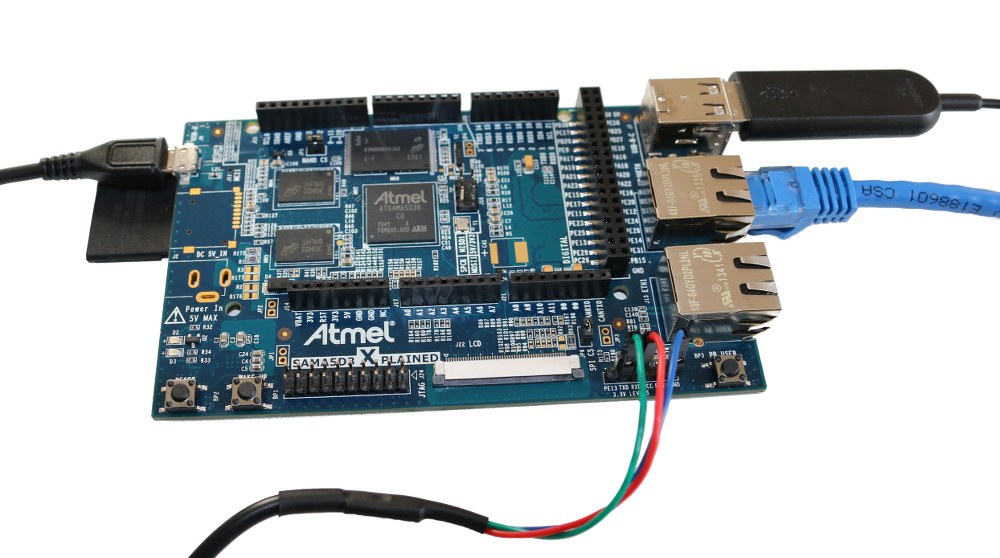
\includegraphics[height=5cm]{../slides/xplained-board/xplained-board.png}
  \end{center}
}

\section{Half day 1}

\feagendaonecolumn
{Lecture - Introduction to embedded Linux}
{
  \begin{itemize}
  \item Advantages of Linux versus traditional embedded operating systems.
        Reasons for choosing Linux.
  \item Global picture: understanding the general architecture of an
        embedded Linux system. Overview of the major components in a typical
        system.
  \end{itemize}
  {\em The rest of the course will study each of these components in detail.}
}

\feagendatwocolumn
{Lecture - Embedded Linux development environment}
{
  \begin{itemize}
  \item Operating system and tools to use on the development
        workstation for embedded Linux development.
  \item Desktop Linux usage tips.
  \end{itemize}
}
{Lecture - Cross-compiling toolchain and C library}
{
  \begin{itemize}
  \item What's inside a cross-compiling toolchain
  \item Choosing the target C library
  \item What's inside the C library
  \item Ready to use cross-compiling toolchains
  \item Building a cross-compiling toolchain with automated tools.
  \end{itemize}
}

\section{During spare time between sessions}

\feagendaonecolumn
{Optional lab - Cross compiling toolchain}
{
  \begin{itemize}
  \item Configuring Crosstool-NG
  \item Executing it to build a custom uClibc toolchain.
  \end{itemize}
}

\section{Half day 2}

\feagendaonecolumn
{Solution demo - Cross compiling toolchain}
{
  {\em Corresponding to the above optional lab}
}

\feagendaonecolumn
{Lecture - Bootloaders}
{
  \begin{itemize}
  \item Available bootloaders
  \item Bootloader features
  \item Installing a bootloader
  \item Detailed study of U-Boot
  \end{itemize}
}

\feagendaonecolumn
{Lecture - Linux kernel}
{
  \begin{itemize}
  \item Role and general architecture of the Linux kernel
  \item Features available in the Linux kernel,
        with a focus on features useful for embedded systems
  \item Kernel user interface
  \item Getting the sources
  \item Understanding Linux kernel versions.
  \item Using the patch command
  \end{itemize}
}

\feagendaonecolumn
{Lecture – Configuring and compiling a Linux kernel}
{
  \begin{itemize}
  \item Kernel configuration.
  \item Using ready-made configuration files for specific
    architectures and boards.
  \item Kernel compilation.
  \item Generated files.
  \item Using kernel modules
  \end{itemize}
}

\section{During spare time between sessions}

\feagendaonecolumn
{Optional lab - Bootloader and U-boot}
{
  {\em Using the QEMU emulated ARM Vexpress A9 board}
  \begin{itemize}
  \item Configure U-Boot for your virtual board
  \item Build U-Boot with your new toolchain
  \item Start U-Boot directly from QEMU and test it.
  \item Store the U-Boot environment in an emulated SD card
  \item Setup networking between your PC and the QEMU emulated machine
  \item Setup tftp for transferring files between the host and U-Boot
        in QEMU
  \end{itemize}
}

\feagendaonecolumn
{Optional lab - Kernel sources}
{
  \begin{itemize}
  \item Downloading kernel sources
  \item Applying kernel patches
  \end{itemize}
}

\feagendaonecolumn
{Optional lab - Kernel cross-compiling and booting}
{
  {\em Using the QEMU emulated ARM Vexpress A9 board}
  \begin{itemize}
  \item Configuring the Linux kernel and cross-compiling it for the ARM board.
  \item Boot Linux from U-Boot through tftp
  \item Automate the boot sequence in U-Boot
  \end{itemize}
}

\section{Half day 3}

\feagendaonecolumn
{Solution demo - Bootloader and U-boot}
{
  {\em Using the Microchip SAMA5D3 Xplained board}
  \begin{itemize}
  \item Set up serial communication with the board.
  \item Configure, compile and install the first-stage bootloader
        and U-Boot on the Xplained board.
  \item Become familiar with U-Boot environment and commands.
  \item Set up TFTP communication with the board. Use TFTP U-Boot commands.
  \end{itemize}
}

\feagendaonecolumn
{Solution demo - Kernel sources}
{
  \begin{itemize}
  \item Downloading kernel sources
  \item Apply kernel patches
  \end{itemize}
}

\feagendaonecolumn
{Solution demo - Kernel cross-compiling and booting}
{
  {\em Using the Microchip Xplained board}
  \begin{itemize}
  \item Configuring the Linux kernel and cross-compiling it for the ARM board.
  \item Downloading your kernel on the board through U-boot's tftp client.
  \item Booting your kernel from RAM.
  \item Copying the kernel to flash and booting it from this location.
  \item Storing boot parameters in flash and automating kernel booting from flash.
  \end{itemize}
}

\feagendaonecolumn
{Lecture – Root filesystem in Linux}
{
  \begin{itemize}
  \item Filesystems in Linux.
  \item Role and organization of the root filesystem.
  \item Location of the root filesystem: on storage, in memory,
        from the network.
  \item Device files, virtual filesystems.
  \item Contents of a typical root filesystem.
  \end{itemize}
}

\feagendaonecolumn
{Lecture - BusyBox}
{
  \begin{itemize}
  \item Detailed overview. Detailed features.
  \item Configuration, compiling and deploying.
  \end{itemize}
}

\feagendaonecolumn
{Lecture - Block filesystems}
{
  \begin{itemize}
  \item Filesystems for block devices.
  \item Usefulness of journaled filesystems.
  \item Read-only block filesystems.
  \item RAM filesystems.
  \item How to create each of these filesystems.
  \item Suggestions for embedded systems.
  \end{itemize}
}

\newpage
\section{During spare time between sessions}

\feagendaonecolumn
{Optional lab – Tiny root filesystem built from scratch with BusyBox}
{
  {\em Using the QEMU emulated ARM Vexpress A9 board}
  \begin{itemize}
  \item Now build a basic root filesystem from scratch for your ARM system
  \item Setting up a kernel to boot your system on a host
        directory exported by NFS
  \item Passing kernel command line parameters to boot on NFS
  \item Creating the full root filesystem from scratch.
        Populating it with BusyBox based utilities.
  \item Creating device files and booting the virtual system.
  \item System startup using BusyBox /sbin/init
  \item Using the BusyBox http server.
  \item Controlling the target from a web browser on the PC host.
  \item Setting up shared libraries on the target and compiling
        a sample executable.
  \end{itemize}
}

\section{Half day 4}

\feagendaonecolumn
{Solution demo – Tiny root filesystem built from scratch with BusyBox}
{
  {\em Implementing the same functionality as on QEMU but with the Microchip Xplained board}
}

\feagendaonecolumn
{Lecture - Flash filesystems}
{
  \begin{itemize}
  \item The Memory Technology Devices (MTD) filesystem.
  \item Filesystems for MTD storage: JFFS2, Yaffs2, UBIFS.
  \item Kernel configuration options
  \item MTD storage partitions.
  \item Focus on today's best solution, UBI and UBIFS:
	preparing, flashing and using UBI images.
  \end{itemize}
}

\section{During spare time between sessions}

\feagendaonecolumn
{Optional lab - Block filesystems}
{
  {\em Using the QEMU emulated ARM Vexpress A9 board}
  \begin{itemize}
  \item Booting your system with a mix of filesystems on MMC/SD storage: SquashFS for
	applications, ext4 for configuration and user data, and
	tmpfs for temporary system files.
  \end{itemize}
}

\section{Half day 5}

\feagendaonecolumn
{Solution demo - Block filesystems}
{
  {\em Implementing the same functionality as on QEMU but with the Microchip Xplained board}
}

\feagendaonecolumn
{Demo – Flash filesystems}
{
  {\em Using the SAMAD3 Xplained ARM board}
  \begin{itemize}
  \item Defining partitions in U-Boot for your internal
        flash storage instead of using raw offsets.
  \item Sharing these definitions with Linux.
  \item Creating a UBI image on your workstation, flashing
        it from U-Boot and booting your system on one of
        the UBI volumes with UBIFS.
  \end{itemize}
}

\feagendatwocolumn
{Lecture – Leveraging existing open-source components in your system}
{
  \begin{itemize}
  \item Reasons for leveraging existing components.
  \item Find existing free and open source software components.
  \item Choosing the components.
  \item The different free software licenses and their requirements.
  \item Overview of well-known typical components used in
        embedded systems: graphical libraries and systems
        (framebuffer, Gtk, Qt, etc.), system utilities,
        network libraries and utilities, multimedia libraries, etc.
  \item System building: integration of the components.
  \end{itemize}
}
{Lecture – Cross-compiling applications and libraries}
{
  \begin{itemize}
  \item Configuring, cross-compiling and installing applications and libraries.
  \item Details about the build system used in most open-source components.
  \item Overview of the common issues found when using these components.
  \end{itemize}
}

\section{During spare time between sessions}

\feagendaonecolumn
{Optional lab – Cross-compiling applications and libraries}
{
  {\em Using the QEMU emulated ARM Vexpress A9 board}
  \begin{itemize}
  \item Building a system with audio libraries and a sound player application.
  \item Manual compilation and installation of several free software packages.
  \item Learning about common techniques and issues.
  \end{itemize}
}

\section{Half day 6}

\feagendaonecolumn
{Solution demo – Cross-compiling applications and libraries}
{
  {\em Implementing the same functionality as on QEMU but with the Microchip Xplained board}
}

\feagendaonecolumn
{Lecture - Embedded system building tools}
{
  \begin{itemize}
  \item Review of existing system building tools.
  \item Buildroot example.
  \end{itemize}
}

\feagendaonecolumn
{Lecture - Application development and debugging}
{
  \begin{itemize}
  \item Programming languages and libraries available.
  \item Overview of the C library features for application development.
  \item Build system for your application,
        how to use existing libraries in your application.
  \item Source browsers and Integrated Development Environments (IDEs).
  \item Debuggers. Debugging remote applications with gdb and gdbserver.
        Post-mortem debugging with core files.
  \item Code checkers, memory checkers, profilers.
  \end{itemize}
}

\section{During spare time between sessions}

\feagendaonecolumn
{Optional lab - System build with Buildroot}
{
  {\em Using the QEMU emulated ARM Vexpress A9 board}
  \begin{itemize}
  \item Using Buildroot to rebuild the same system as in the previous lab.
  \item Seeing how easier it gets.
  \end{itemize}
}

\feagendaonecolumn
{Optional lab – Application development and debugging}
{
  {\em On the Microchip Xplained board}
  \begin{itemize}
  \item Develop and compile an application relying on the ncurses library
  \item Using strace, ltrace and gdbserver to debug a crappy application
        on the remote system.
  \end{itemize}
}

\section{Half day 7}

\feagendaonecolumn
{Solution demo - System build with Buildroot}
{
  {\em Implementing the same functionality as on QEMU but with the Microchip Xplained board}
}

\feagendaonecolumn
{Solution demo - Application development and debugging}
{
  {\em Implementing the same functionality as on QEMU but with the Microchip Xplained board}
}

\feagendaonecolumn
{Lecture - Linux and real-time}
{
  {\em Very useful for many kinds of devices, industrial or multimedia systems.}
  \begin{itemize}
  \item Understanding the sources of latency in standard Linux.
  \item Soft real-time solutions for Linux: improvements included
        in the mainline Linux version.
  \item Understanding and using the latest RT preempt patches for
        mainline Linux.
  \item Real-time kernel debugging. Measuring and analyzing latency.
  \item Xenomai, a hard real-time solution for Linux: features, concepts,
        implementation and examples.
  \end{itemize}
}

\feagendaonecolumn
{Demo - Linux latency tests}
{
  \begin{itemize}
  \item Tests performed on the Xplained ARM board.
  \item Latency tests on standard Linux, with preemption options.
  \item Latency tests using the \code{PREEMPT_RT} kernel patchset.
  \item Setting up Xenomai.
  \item Latency tests with Xenomai.
  \end{itemize}
}

\section{Possible extra time}

{\em Extra time (up to 4 hours) may be proposed if the agenda didn't fit in 7 half days,
     according to the time spend answering questions from participants.}

\end{document}
